
\chapter{Sieci głębokie}
Za protoplastę sieci głębokich można uznać zdefiniowany na początku lat dziewięćdziesiątych wielowarstwowy \textbf{neocognitron} Fukushimy, Prawdziwy rozwój tych sieci zawdzięczamy jednak profesorowi LeCun, który zdefiniował podstawową strukturę i algorytm uczący specjalizowanej \textbf{sieci konwolucyjnej} \textit{Convolutional Neural Network} skracanej tradycyjnie do CNN \cite{ossowski2023}. 

\begin{figure}[h]
    	\centering 
            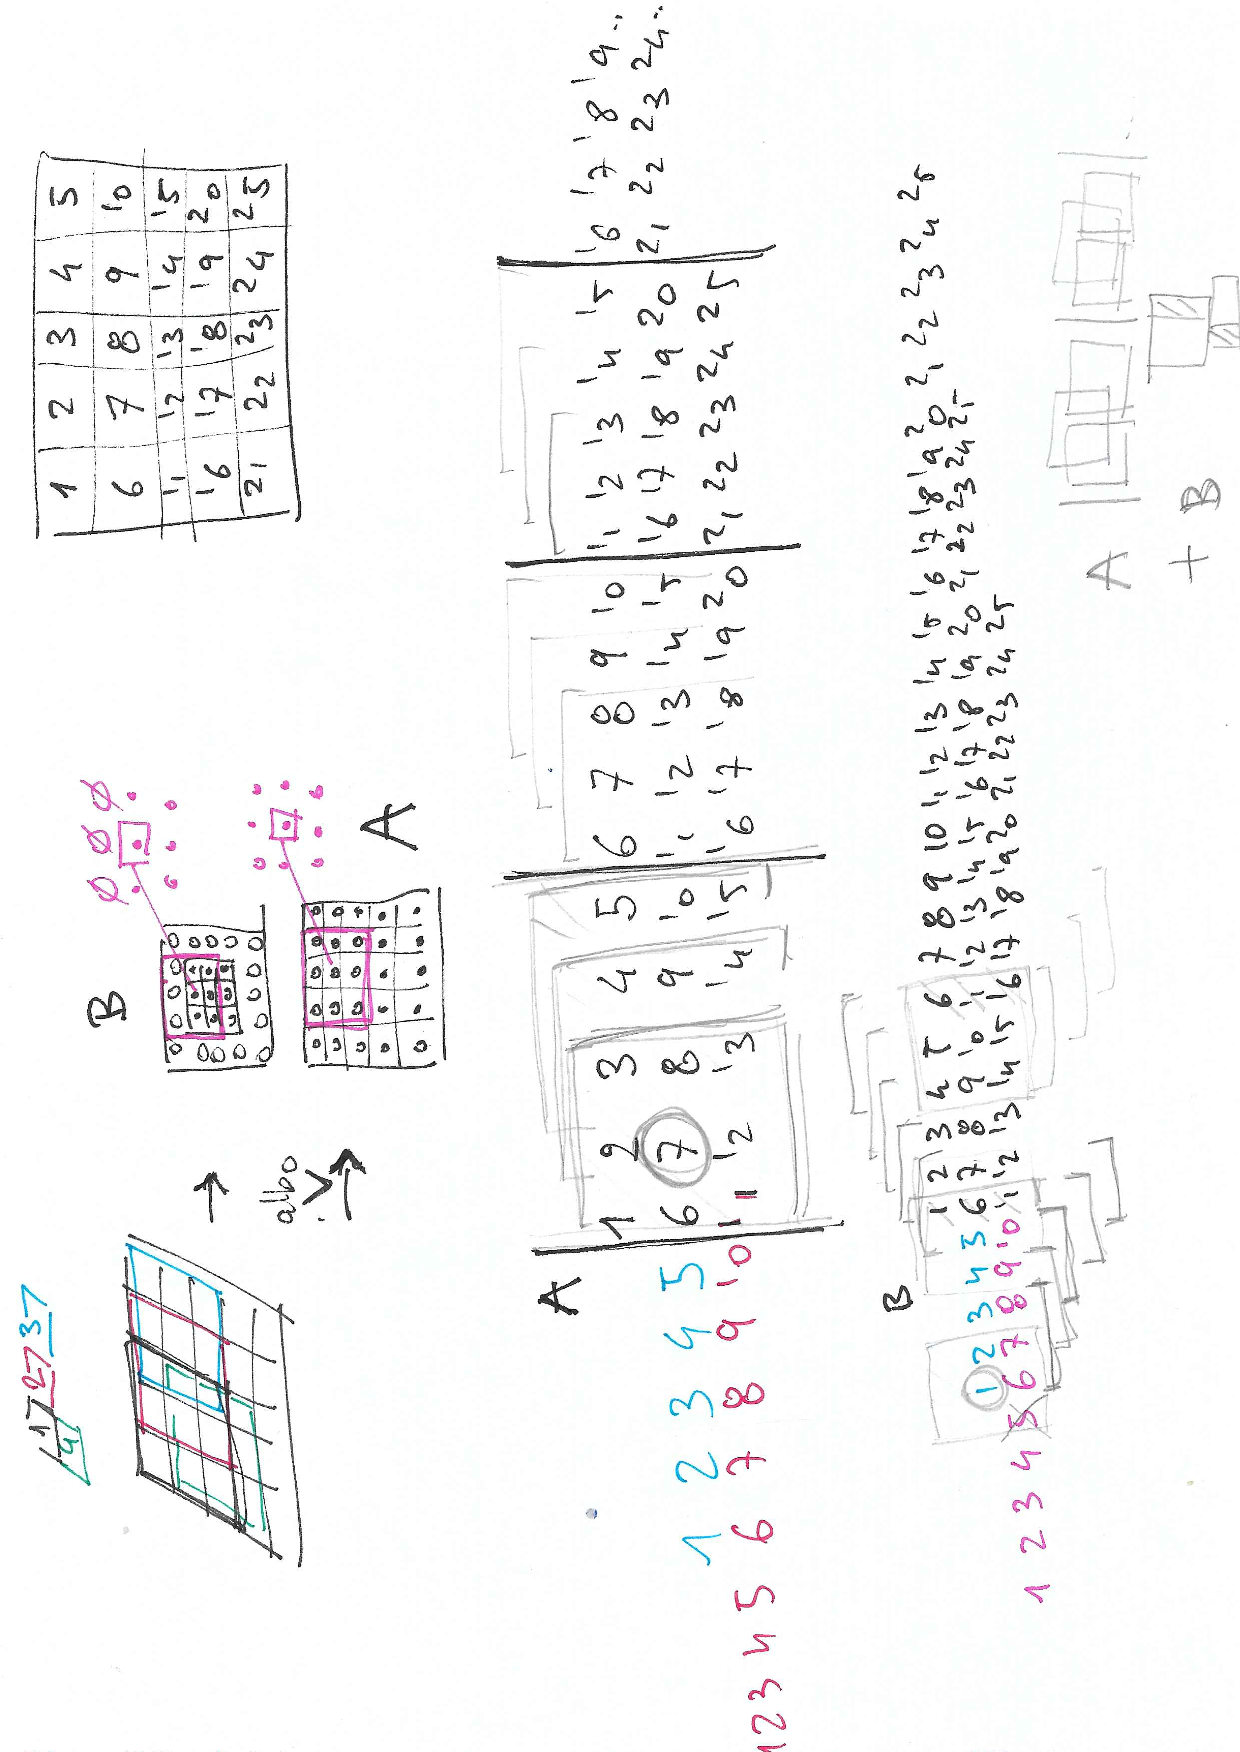
\includegraphics[width=0.70\linewidth]{gfx/scan01.pdf} 
\end{figure} 

\section{CNN}
\begin{lstlisting}
https://www.mathworks.com/matlabcentral/fileexchange/74760-image-classification-using-cnn-with-multi-input-cnn?s_tid=srchtitle_support_results_1_CNN
\end{lstlisting}

\section{Python TensFlow}
..
// derative of convolution \\

https://www.physicsforums.com/threads/how-do-you-derive-the-derivative-of-a-convolution.403002/

https://dsp.stackexchange.com/questions/46746/how-to-evaluate-derivative-of-convolution-integral

https://en.wikipedia.org/wiki/Convolution